% Add \usepackage{tikz,listings} to the manuscript preamble.
% Place the exact UTF-8 prompt at docs/pilot/prompt.txt relative to the project root.
% Include this file at the end of Appendix A with % Add \usepackage{tikz,listings} to the manuscript preamble.
% Place the exact UTF-8 prompt at docs/pilot/prompt.txt relative to the project root.
% Include this file at the end of Appendix A with % Add \usepackage{tikz,listings} to the manuscript preamble.
% Place the exact UTF-8 prompt at docs/pilot/prompt.txt relative to the project root.
% Include this file at the end of Appendix A with % Add \usepackage{tikz,listings} to the manuscript preamble.
% Place the exact UTF-8 prompt at docs/pilot/prompt.txt relative to the project root.
% Include this file at the end of Appendix A with \input{docs/pilot/paper-appendix.tex}.
\subsection*{Classifier inputs and review sequence}
The rule baseline and the LLM each received 15 frozen packets containing
18 excerpts from 17 source URLs. In each packet, the context field was the
original short excerpt. The LLM received the same record, dates and source
metadata as the rules. Reviewers could consult fuller sources. Figure~\ref{fig:morocco-pilot-flow}
shows when the final reference labels were assigned.

\begin{figure}[htbp]
\centering
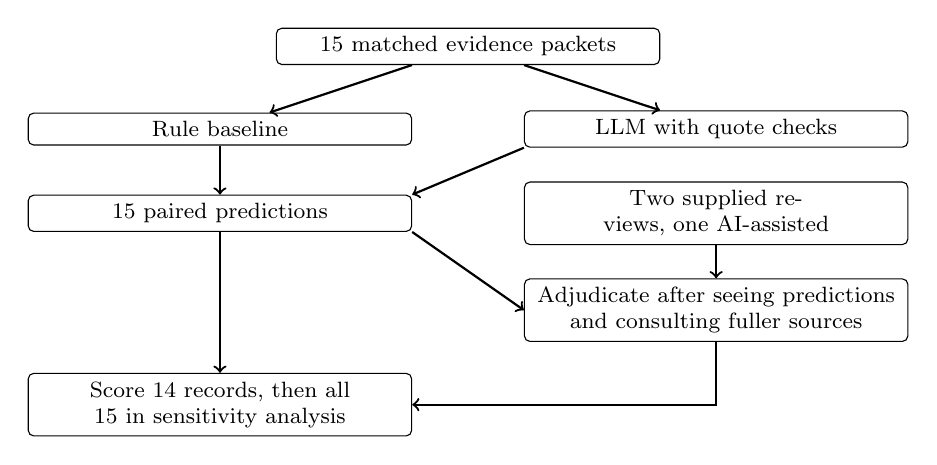
\begin{tikzpicture}[
  x=.01\linewidth,y=1cm,
  box/.style={draw,rounded corners=2pt,align=center,inner xsep=2pt,inner ysep=3pt,
              text width=.39\linewidth,font=\footnotesize},
  arr/.style={->,thick}
]
\node[box] (inputs) at (50,0) {15 matched evidence packets};
\node[box] (rules) at (24,-1.05) {Rule baseline};
\node[box] (llm) at (76,-1.05) {LLM with quote checks};
\node[box] (pred) at (24,-2.12) {15 paired predictions};
\node[box] (review) at (76,-2.12) {Two supplied reviews, one AI-assisted};
\node[box] (labels) at (76,-3.35) {Adjudicate after seeing predictions and consulting fuller sources};
\node[box] (score) at (24,-4.55) {Score 14 records, then all 15 in sensitivity analysis};
\draw[arr] (inputs) -- (rules);
\draw[arr] (inputs) -- (llm);
\draw[arr] (rules) -- (pred);
\draw[arr] (llm.south west) -- (pred.north east);
\draw[arr] (review) -- (labels);
\draw[arr] (pred.south east) -- (labels.west);
\draw[arr] (pred) -- (score);
\draw[arr] (labels.south) |- (score.east);
\end{tikzpicture}
\caption{Retrospective classification and scoring. The rules and LLM made
their predictions before the final reference labels were settled.}
\label{fig:morocco-pilot-flow}
\end{figure}

\subsection*{Exact classifier instructions}
We sent the instructions below with each request to
\texttt{gpt-4.1-mini-2025-04-14}. Each request included one evidence
packet as JSON and required a response conforming to the
\texttt{deployment\_stage} schema. The instructions assumed screened
eligibility. We later excluded R01 from the primary comparison.

\lstinputlisting[basicstyle=\ttfamily\footnotesize,breaklines=true,
  breakatwhitespace=true,columns=fullflexible,keepspaces=true,
  showstringspaces=false]{docs/pilot/prompt.txt}
.
\subsection*{Classifier inputs and review sequence}
The rule baseline and the LLM each received 15 frozen packets containing
18 excerpts from 17 source URLs. In each packet, the context field was the
original short excerpt. The LLM received the same record, dates and source
metadata as the rules. Reviewers could consult fuller sources. Figure~\ref{fig:morocco-pilot-flow}
shows when the final reference labels were assigned.

\begin{figure}[htbp]
\centering
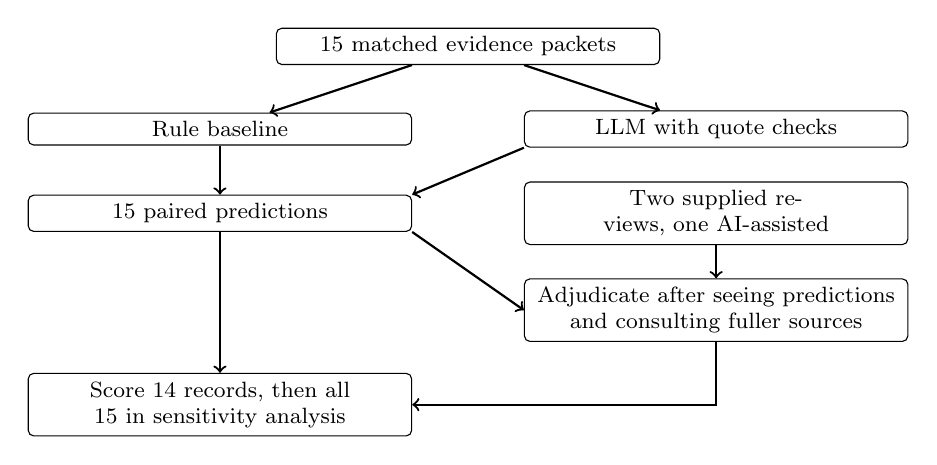
\begin{tikzpicture}[
  x=.01\linewidth,y=1cm,
  box/.style={draw,rounded corners=2pt,align=center,inner xsep=2pt,inner ysep=3pt,
              text width=.39\linewidth,font=\footnotesize},
  arr/.style={->,thick}
]
\node[box] (inputs) at (50,0) {15 matched evidence packets};
\node[box] (rules) at (24,-1.05) {Rule baseline};
\node[box] (llm) at (76,-1.05) {LLM with quote checks};
\node[box] (pred) at (24,-2.12) {15 paired predictions};
\node[box] (review) at (76,-2.12) {Two supplied reviews, one AI-assisted};
\node[box] (labels) at (76,-3.35) {Adjudicate after seeing predictions and consulting fuller sources};
\node[box] (score) at (24,-4.55) {Score 14 records, then all 15 in sensitivity analysis};
\draw[arr] (inputs) -- (rules);
\draw[arr] (inputs) -- (llm);
\draw[arr] (rules) -- (pred);
\draw[arr] (llm.south west) -- (pred.north east);
\draw[arr] (review) -- (labels);
\draw[arr] (pred.south east) -- (labels.west);
\draw[arr] (pred) -- (score);
\draw[arr] (labels.south) |- (score.east);
\end{tikzpicture}
\caption{Retrospective classification and scoring. The rules and LLM made
their predictions before the final reference labels were settled.}
\label{fig:morocco-pilot-flow}
\end{figure}

\subsection*{Exact classifier instructions}
We sent the instructions below with each request to
\texttt{gpt-4.1-mini-2025-04-14}. Each request included one evidence
packet as JSON and required a response conforming to the
\texttt{deployment\_stage} schema. The instructions assumed screened
eligibility. We later excluded R01 from the primary comparison.

\lstinputlisting[basicstyle=\ttfamily\footnotesize,breaklines=true,
  breakatwhitespace=true,columns=fullflexible,keepspaces=true,
  showstringspaces=false]{docs/pilot/prompt.txt}
.
\subsection*{Classifier inputs and review sequence}
The rule baseline and the LLM each received 15 frozen packets containing
18 excerpts from 17 source URLs. In each packet, the context field was the
original short excerpt. The LLM received the same record, dates and source
metadata as the rules. Reviewers could consult fuller sources. Figure~\ref{fig:morocco-pilot-flow}
shows when the final reference labels were assigned.

\begin{figure}[htbp]
\centering
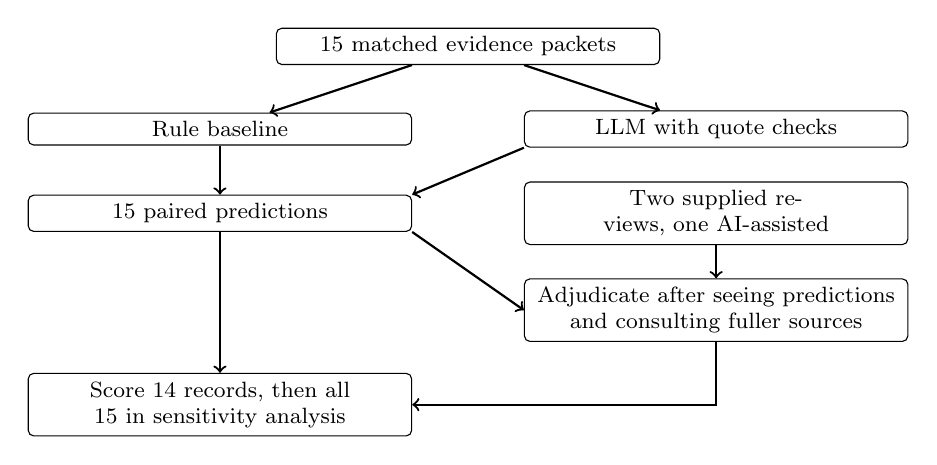
\begin{tikzpicture}[
  x=.01\linewidth,y=1cm,
  box/.style={draw,rounded corners=2pt,align=center,inner xsep=2pt,inner ysep=3pt,
              text width=.39\linewidth,font=\footnotesize},
  arr/.style={->,thick}
]
\node[box] (inputs) at (50,0) {15 matched evidence packets};
\node[box] (rules) at (24,-1.05) {Rule baseline};
\node[box] (llm) at (76,-1.05) {LLM with quote checks};
\node[box] (pred) at (24,-2.12) {15 paired predictions};
\node[box] (review) at (76,-2.12) {Two supplied reviews, one AI-assisted};
\node[box] (labels) at (76,-3.35) {Adjudicate after seeing predictions and consulting fuller sources};
\node[box] (score) at (24,-4.55) {Score 14 records, then all 15 in sensitivity analysis};
\draw[arr] (inputs) -- (rules);
\draw[arr] (inputs) -- (llm);
\draw[arr] (rules) -- (pred);
\draw[arr] (llm.south west) -- (pred.north east);
\draw[arr] (review) -- (labels);
\draw[arr] (pred.south east) -- (labels.west);
\draw[arr] (pred) -- (score);
\draw[arr] (labels.south) |- (score.east);
\end{tikzpicture}
\caption{Retrospective classification and scoring. The rules and LLM made
their predictions before the final reference labels were settled.}
\label{fig:morocco-pilot-flow}
\end{figure}

\subsection*{Exact classifier instructions}
We sent the instructions below with each request to
\texttt{gpt-4.1-mini-2025-04-14}. Each request included one evidence
packet as JSON and required a response conforming to the
\texttt{deployment\_stage} schema. The instructions assumed screened
eligibility. We later excluded R01 from the primary comparison.

\lstinputlisting[basicstyle=\ttfamily\footnotesize,breaklines=true,
  breakatwhitespace=true,columns=fullflexible,keepspaces=true,
  showstringspaces=false]{docs/pilot/prompt.txt}
.
\subsection*{Classifier inputs and review sequence}
The rule baseline and the LLM each received 15 frozen packets containing
18 excerpts from 17 source URLs. In each packet, the context field was the
original short excerpt. The LLM received the same record, dates and source
metadata as the rules. Reviewers could consult fuller sources. Figure~\ref{fig:morocco-pilot-flow}
shows when the final reference labels were assigned.

\begin{figure}[htbp]
\centering
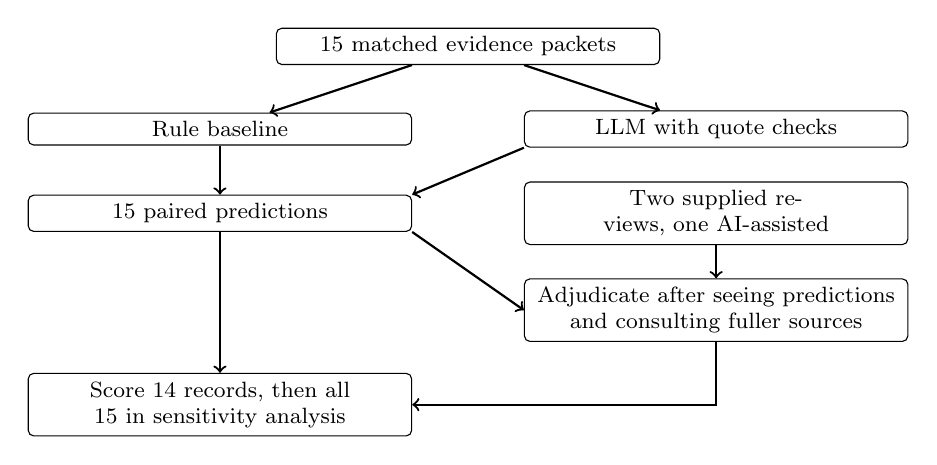
\begin{tikzpicture}[
  x=.01\linewidth,y=1cm,
  box/.style={draw,rounded corners=2pt,align=center,inner xsep=2pt,inner ysep=3pt,
              text width=.39\linewidth,font=\footnotesize},
  arr/.style={->,thick}
]
\node[box] (inputs) at (50,0) {15 matched evidence packets};
\node[box] (rules) at (24,-1.05) {Rule baseline};
\node[box] (llm) at (76,-1.05) {LLM with quote checks};
\node[box] (pred) at (24,-2.12) {15 paired predictions};
\node[box] (review) at (76,-2.12) {Two supplied reviews, one AI-assisted};
\node[box] (labels) at (76,-3.35) {Adjudicate after seeing predictions and consulting fuller sources};
\node[box] (score) at (24,-4.55) {Score 14 records, then all 15 in sensitivity analysis};
\draw[arr] (inputs) -- (rules);
\draw[arr] (inputs) -- (llm);
\draw[arr] (rules) -- (pred);
\draw[arr] (llm.south west) -- (pred.north east);
\draw[arr] (review) -- (labels);
\draw[arr] (pred.south east) -- (labels.west);
\draw[arr] (pred) -- (score);
\draw[arr] (labels.south) |- (score.east);
\end{tikzpicture}
\caption{Retrospective classification and scoring. The rules and LLM made
their predictions before the final reference labels were settled.}
\label{fig:morocco-pilot-flow}
\end{figure}

\subsection*{Exact classifier instructions}
We sent the instructions below with each request to
\texttt{gpt-4.1-mini-2025-04-14}. Each request included one evidence
packet as JSON and required a response conforming to the
\texttt{deployment\_stage} schema. The instructions assumed screened
eligibility. We later excluded R01 from the primary comparison.

\lstinputlisting[basicstyle=\ttfamily\footnotesize,breaklines=true,
  breakatwhitespace=true,columns=fullflexible,keepspaces=true,
  showstringspaces=false]{docs/pilot/prompt.txt}
